\documentclass{beamer}
\usepackage{etex}
\usetheme{Antibes}
\usepackage{amssymb,amsmath,amsthm}
\usepackage{graphicx}
\usepackage{caption}
\usepackage{subfig}
\newcommand{\bn}{\begin{enumerate}[i)]}
\newcommand{\en}{\end{enumerate}}
\newcommand{\im}{\item}
\newcommand{\CPT}[1]{\large{\textbf{CHAPTER #1}}}
\newcommand{\ir}[1]{\textbf{Remark #1}}
\newcommand{\ith}[1]{\textbf{Theorem #1}}
\newcommand{\idf}[1]{\textbf{Definition #1}}
\newcommand{\iex}[1]{\textbf{Example #1}}

%\definecolor{cardinal}{rgb}{0.77, 0.12, 0.23}
%\usecolortheme[named=cardinal]{structure}
%\setbeamercolor{block title}{bg=cardinal,fg=black}
 \usepackage{tikz}
 \usetikzlibrary{patterns,snakes,plotmarks}
 \usepackage{multirow}
% \usetikzlibrary{shadows}
\usepackage{epstopdf}
\usepackage{nicefrac}
\usepackage{lmodern}
\usepackage{pgfplots}
\usepackage{qtree}
\newcommand*{\Scale}[2][4]{\scalebox{#1}{\ensuremath{#2}}}%
\DeclareCaptionLabelSeparator{horse}{:\,\,} % change according to your needs
\captionsetup{
  labelsep = horse,
  figureposition = bottom % used to get the correct vertical space between the figure and the caption
}
\setbeamertemplate{caption}[numbered]
\setbeamertemplate{items}[circle]
\setbeamertemplate{enumerate items}[square]
\theoremstyle{definition}
\newtheorem*{exs}{Examples}
\newtheorem{ex}{Example}
\newtheorem*{exc}{Exercise}
%\usepackage{booktabs}
\setlength{\parindent}{0pt}
%\setbeameroption{show notes}
 \setbeamerfont{note page}{size=\tiny}
%\setbeamertemplate{note page}[plain]
%\setbeameroption{show only notes}
\title{Math 629 - Survival Analysis \\ Chapter 4: Evaluating the Proportional Hazards Assumption}
\author{Drew Lazar}
\institute{Ball State University}
\date{\today}

\begin{document}
\begin{frame}
    \titlepage
\end{frame}



\section{Chapter 4}
\begin{frame}
\frametitle{Overview of Evaluating PH Assumption}
\begin{block}{Approaches for assessing PH assumption}
\begin{enumerate}
\item Graphical techniques
\begin{enumerate}[i.]
\item Inspect $-\ln(-\ln(\hat{S}))$ survival curves for specifications of covariates of interest.
\item Comparing observed (stratified KM) and expected (Cox PH model) survival curves.
\end{enumerate}
\item Goodness of fit (GOF) techniques. Conduct test of $H_0: \text{Cox PH assumption met}$ and get a $p$-value.
\item Use time-dependent variables in an extended Cox PH model. Test for interaction between these variables and covariates.
\end{enumerate}
\end{block}
\end{frame}
\begin{frame}
\frametitle{Graphical Approaches}
\begin{block}{Log-Log Plots}
Assume Cox PH is met so that
\[ S(t,X) = S_0(t)^{\exp(X'\beta)} \text{ for some }  \beta \in \mathbb{R}^{p\times1}
\]
Then we have
\begin{align*}
&\ln( S(t,X)) = \exp(X'\beta)\ln(S_0(t)) \\
&\implies -\ln(-\ln(S(t,X))) = -\ln(\ln(-S_0(t))) - X'\beta
\end{align*}
\end{block}
\end{frame}

\begin{frame}
\frametitle{Graphical Approaches (cont'd)}
\begin{block}{Log-Log Plots}
Thus, if population satisfies Cox PH model, for any $X$ and $X^*$,
\begin{align*}
&-\ln(-\ln(S(t,X)))- (-\ln(-\ln(S(t,X^*)))) = \\
&-X'\beta - (-{X^*}'\beta) =(X^*-X)'\beta
\end{align*}
\end{block}
As this expression does not involve time, the  $-\ln(-\ln)$ plots of our survival curves for $X$ and $X^*$, respectively, should be at the same distance throughout the study and their graphs should be parallel. $-\ln(-\ln)$ plots of good estimates, $\hat{S}(t,X)$ and $\hat{S}(t,X^*)$, should exhibit the same behavior.
\end{frame}

\begin{frame}
\frametitle{Graphical Approaches (cont'd)}
\begin{block}{Problem 4.1 - Log-Log Plots}
For the Remission data, test the Cox PH assumption by using log-log plots and by considering the covariates ``one at a time''.
\begin{enumerate}
\item Test Cox Ph assumption for TR.
\item Test the Cox Ph assumption of LogWBC. First statify LogWbc with low - 1.45 to 2.30, med - 2.31 to 3.00, high 3.01 to 5.00.
\item Test the Cox Ph for Sex.
\end{enumerate}
\end{block}
\end{frame}

\begin{frame}
\frametitle{Graphical Approaches (cont'd)}
\begin{block}{Considerations about Log-Log Plots}
\begin{enumerate}
\item  One might ask "How parallel is parrel enough?". Determining parallelism is based on inspection and is subjective. 
\item  For continuous variables such as LogWBC once must choose ``cut-points''. Want many cut-points, but if choose too many data ``thins'' out.
\item  To fully test Cox PH model must choose every combination of classes of covariates. Data might ``thin out'' in this case so test is not reliable (see next slide).  
\end{enumerate}
\end{block}
\end{frame}


\begin{frame}
\frametitle{Graphical Approaches (cont'd)}
\begin{block}{Considerations about Log-Log Plots (cont'd)}
\begin{columns}
    \begin{column}{0.48\textwidth}
        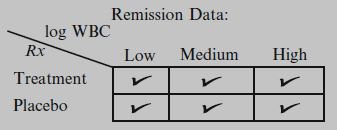
\includegraphics[width =\textwidth, height=4cm]{CH4_loglogMC.JPG}
    \end{column}
    \hspace{-10pt}
    \begin{column}{0.48\textwidth}
         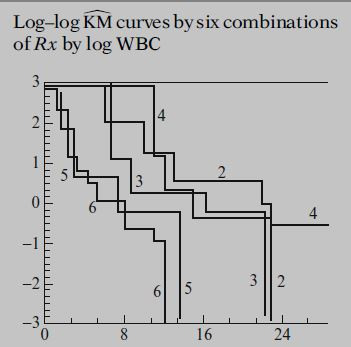
\includegraphics[width =\textwidth, height=5.5cm]{Ch4_loglog6.JPG}
          Plot suggests Cox PH not satisfied, but unreliable. 
    \end{column}
\end{columns}
\end{block}
\end{frame}

\begin{frame}
\frametitle{Graphical Approaches (cont'd)}
\begin{block}{Problem 4.2 - Alternative approach to Log-Log plots} 
\begin{itemize}
\item Rather than use KM plots on strata, we can fit Cox PH models using covariates that already satisfy the PH assumption. 
\item These PH models are fit on strata of covariates we are testing.
\item We then check log-log plots of estimated survival curves from different stata.  We use representative values (eg. overall mean) of covariates which we included in Cox PH model.
\end{itemize}
Use the approach above, assuming LogWBC satisfies the Cox PH model, to test whether TR satisfies the Cox PH assumption.   
\end{block}
\end{frame}




\end{document} 